% Set the author and title of the compiled pdf
\hypersetup{
	pdftitle = {\Title},
	pdfauthor = {\Author}
}

\section{Introduction}

Performance is always an attribute in high demand in computer systems. Even
though processors have become so much more powerful over the last half century,
there's still loads of stuff that we cannot do with current technology, such as
synthesising HD video in realtime, or computing realistic game physics.

Since 2004/5, companies haven't been able to increase the speed of
microprocessors at such a rapid rate due to physical limits, such as power
dissipation and device variability. Our devices are still getting faster, but
now architecture and the design of systems play a larger role in making stuff
run faster. An example of this include making computation more parallel.

\section{Caches}

Not all technology has improved at the same relative speed. CPU's have become
over three orders of magnitude faster over the past thirty years, but memory has
increased by only one order of magnitude. This is problematic, since it means
that we need to reconcile this gap in order to achieve efficient computation.

Processor caching is used to let the processor do useful computation while
it's also waiting on the memory. Modern processors couldn't perform anywhere
near how fast they do now without equally modern caching techniques, since the
imbalance between the CPU and main memory is so high.

Caches (in general) provide a limited, but very fast local space for the CPU to
use. They are used in lots of places all over computer science, including web
browsers, mobile phone UI's etc. Likewise, a processor cache is a temporary
store for frequently used memory locations.

The principle of locality is what makes caches work for processors, which is
that the CPU will only use a small subset of memory over a short period of time.
If this subset of memory can be loaded into the cache, then the computation can
be sped up significantly.

Every `cache miss' takes \textit{at least} sixty times longer to execute than a
`cache hit' will (that's assuming there are no page faults etc). Circuit
capacitance is the thing that makes electronic devices slow, and larger
components have a larger capacitance, henceforth large memories are slow.
Dynamic memories (DRAM) store data using capacitance, and are therefore slower
than static memories (SRAM) that work using bistable circuits.

Even the wires between the processor and the memory have a significant
capacitance. Driving signals between chips needs specialised high power
interface circuits. An ideal situation would be to have everything on a single
chip, however current manufacturing limitations prevent this; maybe one day we
will be able to do this.

% TODO: Memory heirachy diagram

\subsection{Why are caches expensive?}

L1, L2 and (usually) L3 caches are SRAM instead of DRAM (which is what main
memory is made from).

SRAM needs six transistors per bit, DRAM needs one.

SRAM is henceforth physically larger, taking up more space on the chip, which is
expensive, since real estate costs money.


\subsection{L1 Cache}

The L1 cache is the first level of caching between the processor and the main
memory. The L1 cache is around 32kb, which is very small in comparison to the
size of the main memory, but this is driven out of necessity, since the cache
needs to be small to be fast. The cache must be able to hold any arbitrary
location in the main memory (since we don't know in advance what the CPU will
want), and henceforth requires specialised structures to implement this.


\subsection{Types of cache}

The cpu will give the cache a full address of a word in memory that it wants to
read. The cache will contain a small selection of values from memory that it has
locally, but will ask the main memory for values that it does not have. This is
called a cache miss and is expensive in comparison to a cache hit.

\subsubsection{Fully associative}

A \textbf{Fully Associative} cache is one where the cache is small (around
32,000 values), but stores both addresses and their corresponding data. The
hardware compares the input address with all of the stored addresses (it does
this in parallel). If the address is found, then the value is returned with no
need to ask the RAM (cache hit), if the value isn't found, then a cache miss
occurs, and the request must go to the main memory.

Caches rely on locality in order to function effectively. There are two types of
locality; temporal locality, which is the principle that if you use an address
once, you may use it again soon (e.g. loops), and spatial locality, where if you
use an address once, you are also likely to use addresses nearby (e.g. arrays).

\marginpar{Spatial locality is exploited better by having a bigger data area in
the cache (returning say 512 bits for every address instead of just one word)}

The cache hit rate is the ratio of cache hits to misses. We need a hit rate of
$98\%$ to hide the speed of memory from the CPU. Instruction hit rates are
usually better than data hit rates (although they are in the same cache
remember). The reason for this is that instructions are accessed in a more
regular pattern, incrementing by one word every time, or looping around etc
(have higher locality).

When we do a cache miss (read), we should add the missed value to the cache. In
order to do this, we need a cache replacement policy to find room in the cache
to put the new value:

\begin{itemize}
	\item LRU - slow, good for hit rates
	\item Round Robin - not as good, easier to implement
	\item Random - Easy to implement, works better than expected.
\end{itemize}

Memory writes are more complicated than reads. If we've already got the value in
the cache, then we change the value in the cache. We can use three write
strategies for cache writes (on hits):

\begin{itemize}
	\item Write through (slow)
	\item Write through + buffer (faster, slow when heavily used)
	\item Copy back on cache replacement.
\end{itemize}

On misses:

\begin{itemize}
	\item We can find a location in the cache, and write to that, then rely on
	copy back later, or write back straight away.
	\item we can skip the cache, and write directly to RAM. Subsequent read will
	add to the cache if necessary (good if you're initialising datastructures
	with zeroes).
\end{itemize}

Fastest one is write allocate or copy back. Main memory and the cache aren't
coherent, which can be a problem for stuff like multiprocessors, autonomous IO
devices etc. This may need cleaning up later.

Each cache line is at least half address and half data, but often, we store more
data per address, so will have 64 bytes of data per 32 bit address.

A fully associative cache is ideal, but this is expensive (in terms of silicon
and power).

\subsubsection{Directly mapped}

We can use standard RAM to create a directly mapped cache, which mimics the
functionality of an ideal cache. Usually, this uses static RAM, which is more
expensive than dynamic RAM, but is faster. The address is divided into two
parts, %TODO: Directly mapepd cache 2,3,4 + direct mapped replacement?

\subsubsection{Set associative}

Set associative caches are a compromise. They comprise of a number of directly
mapped caches operating in parallel. If one matches, we have a hit and select
the appropriate data. This is good because we can have more flexible cache
replacement strategies. In a 4 way, we could choose any one of the four caches
for example. The hit rate of set associative caches improves with the number of
caches, but increasing the number increase the cost.

% Lecture three

\section{Practical caches}

\subsection{Cache control bits}

When the system is started, the cache is empty. We need a bit for each cache
entry to indicate that the data is meaningful (i.e. it isn't just an uninitialised
zero or something). We also need a dirty bit if we're using the `write back'
caching strategy (see above), rather than the `write through' strategy.

\subsection{Exploiting spatial locality}

In order to exploit spatial locality, we need to have a wider `cache line', where
each entry will give you more data than just one word. Each entry tag could
correspond to two, four, eight etc words. Spatial locality says that if we get
one byte, we'll probably want one from close by too.

% TODO: Make image

The lowest bits are used to select the word in the cache line. Most cache lines
are 16 or 32 bytes, which is 4 or 8 32bit words. The data is transferred from
RAM in bursts equal to the width of the line size, using specialised memory
access modes.

%TODO: Explain about more cache line = less number of tags? Is that even right?

The line size is important, since we want to have a line size of multiple words
to exploit spatial locality, but if the line is too big, then parts of it will
never be used. The number of cache misses decreases as you increase the cache
line size, until one point, where the line size will be too long to use all the
words, and then the number of misses will increase.

\subsection{Separate instruction and data caches}

Since instructions and data have different access patterns in memory (but they
are stored in the same memory), we could use different caches for each type of
word, so that the different caches can use different strategies to minimise
misses according to their different access patterns.

\subsection{Multi level caches}

As chips get bigger, in theory, we should build bigger caches to perform better.
However, big caches are slow, and the L1 cache needs to run at processor speed.
We can instead put another cache between the RAM and the L1 cache, and keep the
L1 cache the same size.

The L2 cache is typically sixteen times bigger than the L1 cache, but also four
times slower. It's still ten times faster than RAM though. The L1D and L1I
caches both share the L2 cache.

If a chip has an L3 cache, then it is usually quite large (maybe around 8Mb),
but its performance is only about twice as good as that of RAM.

%TODO: Cache example from slide 16

\subsection{Cache misses}

There are three types of cache misses, called the three C's

\begin{description}
  \item \textbf{Compulsory misses}\\ 
    When we first start the computer, the cache is empty, so until the cache is
    populated, we're going to have a lot of misses.
  \item \textbf{Capacity misses}\\
   Since the cache is limited in size, we can't contain all of the pages for a
   program, so some misses will occur.
  \item \textbf{Conflict misses}\\
    In a direct mapped or set associative cache, there is competition between
    memory locations for places in the cache. If the cache was fully
    associative, then misses due to this wouldn't occur.
\end{description}

\subsection{More cache performance}

%TODO: What happens when IO is memory mapped, does this go through the cache? :o

In order to fill a cache from empty, it takes $\frac{\text{Cache
size}}{\text{Line size}}$ memory accesses. If we multiply this by the time it
takes for a single memory access (say $10\micro\second$), then we can work out
how long it will take to fill the cache (assuming each access is to a unique
memory address). We can derive how many CPU cycles this takes from this.

\subsection{Cache consistency}

We need to make sure that the values stored in the CPU cache are consistent with
those in main memory. There are situations when they can disagree, for example
if IO reads or writes directly to memory (perhaps using DMA), then that value
could be different from whatever is in the cache.

Solutions:
\begin{description}
  \item \textbf{Non-cacheable}\\
    One solution is to make areas of memory that IO can access non-cachable, or
    clear the cache before and after the IO takes place.
  \item \textbf{IO use data cache}\\
    Another is to have the IO go directly through the CPU's L1d (data) cache
    before accessing memory, but this is slow.
  \item \textbf{Snoop on IO activity}\\
    We could have hardware logic that will look at the reads and writes to
    memory from IO and make sure the cache is consistent with memory for those
    addresses.
\end{description}

\subsection{Virtual Addresses}

Since the CPU deals with virtual addresses when accessing memory, and uses a
Translation Lookaside Buffer to derive the correct physical address. However,
which address does the cache store? Does it sit before the TLB, or after it
between the CPU and memory?

If we make addresses go through the TLB before they reach the cache, then this
is slow, since they must pass through extra logic etc before hitting the cache.
However, if we make the cache store virtual addresses, and have the TLB sit
inbetween the cache and memory, this makes snooping hard to implement along with
more functional difficulties.

The answer is to have the TLB operate in parallel to the cache. Since address
translation only affects the high order bits of the cache (the low order bits
are the offset which remains the same). The cache index is selected from the low
order offset bits, and only the tag is changed by address translation.

%TODO: Image goes here (something like in the lecture slide of lecture 4, S15)

\section{Pipelines}

The fetch execution cycle is very repetitive, if we can optimise it, then we can
potentially improve the performance of the system a lot! In very simple systems,
each fetch and execute would take one clock cycle; in detail, it'd look like
this:

\begin{description}
  \item \textbf{Fetch}
    \begin{description}
      \item \textbf{IF} - Fetch instruction from memory
      \item \textbf{ID} - Decode instruction; select registers
    \end{description}
  \item \textbf{Execute}
    \begin{description}
      \item \textbf{EX} - Perform an operation or calculate an address
      \item \textbf{MEM} - Access an operand in memory
      \item \textbf{WB} - Write to registers
    \end{description}
\end{description}

If all that takes one clock cycle, each stage will only be active for about
$\frac{1}{5}$ of a clock cycle, or in other words, each CPU component spends
$80\%$ of its time doing nothing!

If we can get all of those components of the CPU working at the same time, then
we can speed up the clock speed by five times! In order to do this, we can use a
pipeline, with buffers that are flushed every clock cycle inbetween each stage
of the pipeline:

\marginpar{Although we have divided our processor into five stages, you can
split it up into more or less than that (the most simple of which is just to
divide into fetch and execute as we did in \texttt{COMP12111} in the first
year. Modern processors use a lot of stages, maybe around thirty.)}

\begin{figure}[ht]
  \centering
  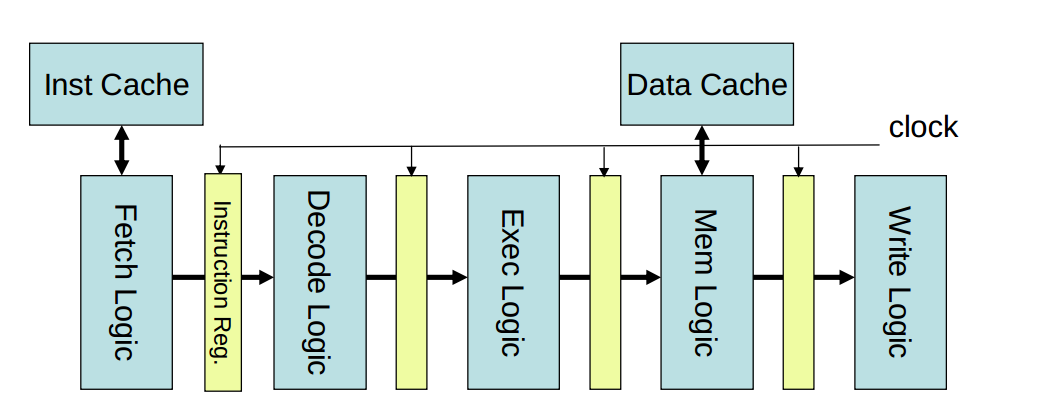
\includegraphics[width=\textwidth]{images/basic-pipeline}
  \caption{Using buffers between the different stages of the pipeline}
  \label{basic-pipeline}
\end{figure}

Now, we can still only execute one instruction per cycle, but we can also
increase our clock speed by five times, since each stage of the pipeline is
isolated by a buffer from the next!

\subsection{Control Transfer Problem}

Using a pipeline is fab if your instructions occur solely in a serial manner,
however, what if your program branches? The processor will only know that a
branch is happening at the \texttt{ID} stage of the pipeline, by which time
we've already fetched the next instruction!

If we come across a branch at the \texttt{ID} stage, then the fetched
instruction at the \texttt{IF} stage will have to be ignored all the way down
the pipeline, so we would waste one clock cycle (or more specifically, we would
waste $\frac{1}{5}$ of the work of five clock cycles!). The ignored instruction
is said to be a \textit{bubble} in the pipeline.

So far, we've assumed that our branch instruction has relies on no conditional
flags. If it did however, we would need to wait until the \texttt{EX} stage of
the pipeline before we knew what the outcome of the conditional evaluation would
be. This has the potential to create two bubbles, since if the branch was to
occur, the instructions at both the \texttt{IF} and \texttt{ID} stages of the
pipeline would have to be ignored.

These bubbles are called \textbf{control hazards}, and they occur when it takes
one or more pipeline stages to detect a branch. Longer pipelines are more likely
to suffer from control hazards more, since more of their pipeline will have been
processed by the time an instruction is detected to be a branch.

\subsubsection{Branch Prediction}

The main technique used to mitigate control hazards is \textbf{branch
prediction}. If we can remember what address a branch directed us to fetch next
from what it did when we executed that branch previously, then we could pre-
emptively load that instruction in the \texttt{IF} stage instead of fetching the
instruction at the PC.

In order to do this, we use a \textbf{branch target buffer}. This maps the
virtual address of one branch instruction onto the virtual address of the
instruction that is branched to, for example:

\begin{table}[ht]
  \centering
  \begin{tabular}{|c|c|}
    \hline
    \textbf{Branch instruction address} & \textbf{Next instruction address} \\ \hline
    \texttt{0xd4f30d2C} & \texttt{0xd4f30d60} \\ \hline
    \texttt{0xd4f30d0f} & \texttt{0xd4f30ddd} \\ \hline
    \multicolumn{1}{c}{\vdots} & \multicolumn{1}{c}{\vdots\vspace{0.2em}}\\ \hline
    \texttt{0xd4f30c4f} & \texttt{0xd4f30d6c} \\ \hline
  \end{tabular}
  \caption{An abstraction of what the datastructure inside a Branch Target
  Buffer could be like}
\end{table}

Now, we will always get unconditional branches right (after we've done it for
the first time), and we will get branches that are part of loops (such as a
\texttt{for} or \texttt{while} loop) right most of the time. If we predict a
branch incorrectly, we just get a bubble like we would if we had no branch
prediction, so it's a win-win situation.

Branch prediction is easy to understand, but implementing it is expensive. In
practice branch predictors use history of each branch (maybe taking the mode of
the last five branches), and the context of the branch (i.e. how did we get to
this point) in order to make a more accurate prediction.

\begin{figure}[ht]
  \centering
  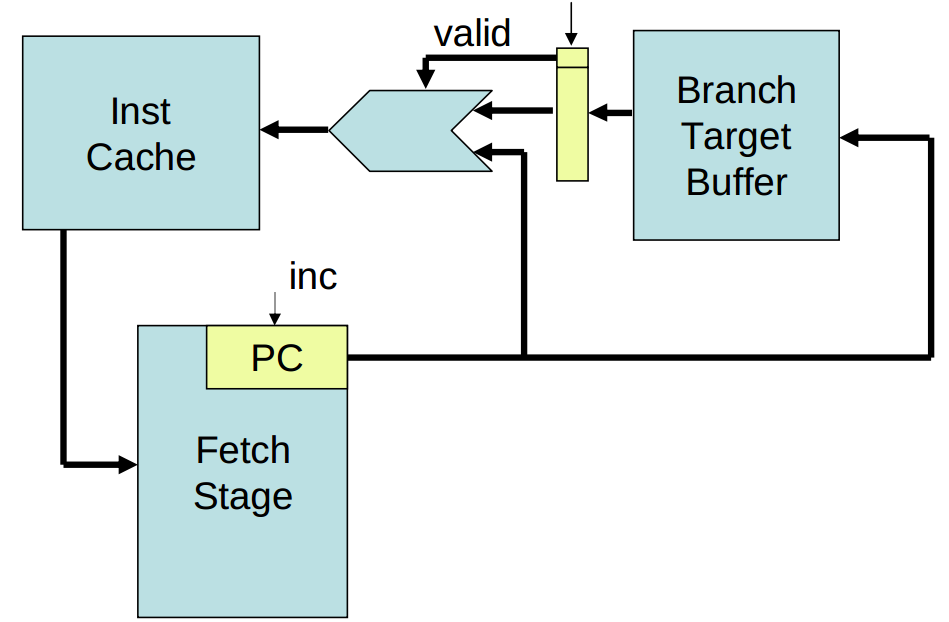
\includegraphics[width=0.5\textwidth]{images/branch-target-buffer}
  \caption{A BTB (Branch Target Buffer) in action}
  % TODO: Work out what this diagram is *actually* showing...
  \label{branch-target-buffer}
\end{figure}

\subsection{Data Hazards}

If we're using a pipeline to process instructions, then we have multiple
instructions at various stages of execution at the same time. This can cause
problems, if multiple instructions that are being executed in parallel operate
on the same resources. For example, if we execute the ARM Assembly code:

\begin{verbatim}
  ADD   R1, R2, R3
  MUL   R0, R1, R1
\end{verbatim}

\marginpar{This problem is called a `data not ready' issue.}

\marginpar{It might take two cycles for a value to be written into a register,
one for \texttt{EX} to complete and push the value into the register bank, and
another for the value to be written into the register.}

Here, the value in \texttt{R0} depends on that of \texttt{R1}. This is a
problem, because we only know the value of \texttt{R1} once the \texttt{ADD}
instruction has finished the \texttt{EX} stage, and the \texttt{MUL} instruction
will get the values from the registers while this is happening in it's
\texttt{ID} stage, henceforth we won't read the correct value of \texttt{R1}.

Two easy solutions to this problem are to:

\begin{itemize}
  \item Detect inter-instruction dependencies in hardware and withhold
  instructions in the decode stage until the data is ready. This creates the
  bubbles that we've worked so hard to avoid with branch prediction though!

  \item Have a compiler detect the dependencies, and have it re-order
  instructions to eliminate them. This is hard to do though, and often results
  in compilers inserting \texttt{NOP} (no operation) instructions that do
  nothing. These act like bubbles anyway, so we don't gain anything here either.
\end{itemize}

Since these are unsatisfactory, we could add extra paths to the pipeline between
the ALU output and the ALU input. They could be activated if there is an
interdependency so that the incorrect result of the \texttt{ID} stage could be
modified before being processed by the ALU.

\begin{figure}[ht]
  \centering
  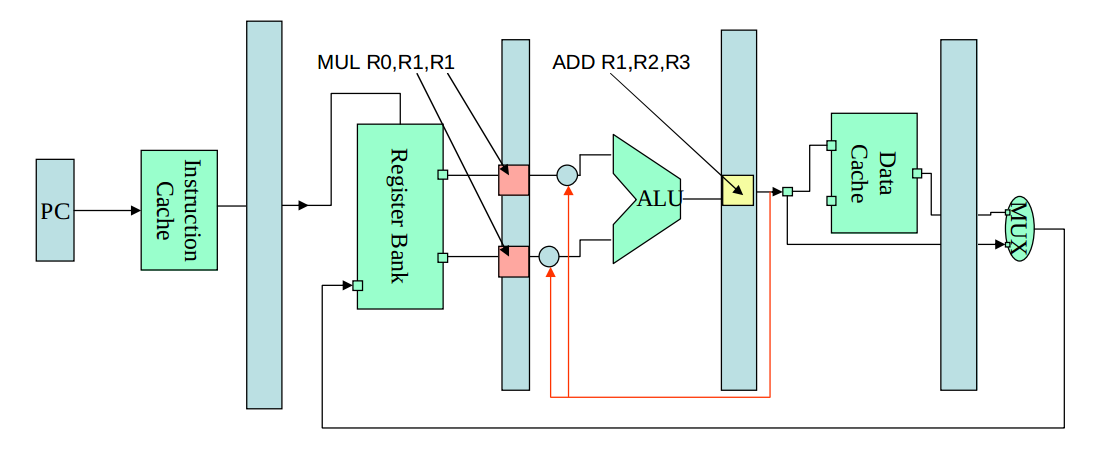
\includegraphics[width=\textwidth]{images/extra-paths}
  \caption{Here, we insert extra paths into the processor so that it can
  mitigate the \texttt{ADD}/\texttt{MUL} dependency.}
  \label{extra-paths}
\end{figure}

What if there is an interdependency with an instruction that might take a while
to execute, such as a memory read (\texttt{LDR})? If we have a program that
does:

\begin{verbatim}
  LDR   R1, [R2, R3]
  MUL   R0, R1, R1
\end{verbatim}

Our path would have to look like this:

\begin{figure}[ht]
  \centering
  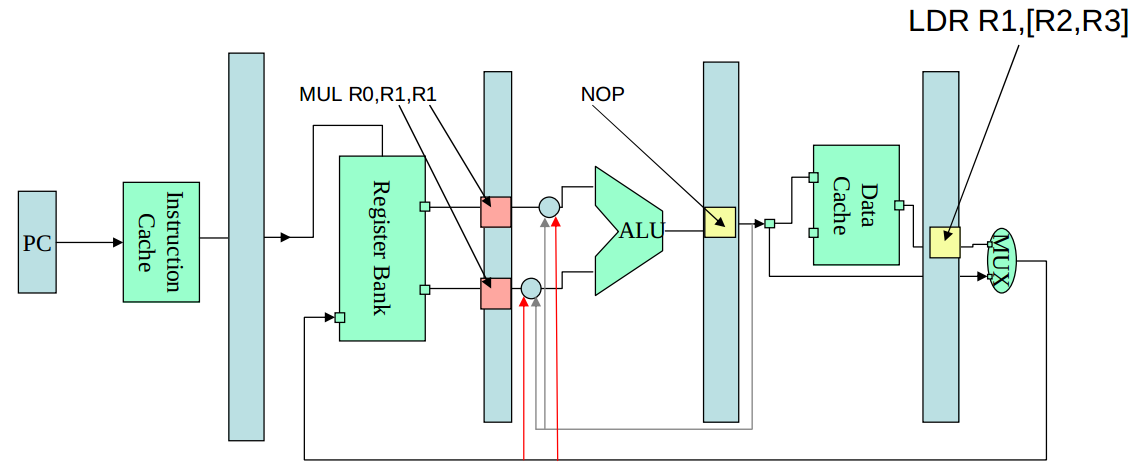
\includegraphics[width=\textwidth]{images/more-extra-paths}
  \caption{In order to cater for the worst case, where we're waiting on a memory
  read, we need even more extra paths.}
  \label{more-extra-paths}
\end{figure}

We want longer pipelines, since we want each stage of the pipeline to do as
little work as possible, taking as little time as possible, so that we can
increase the clock speed. However, as we do that, we will come across more
hazards, and we'll need to put more control paths in to mitigate them.
Eventually, there will come a point where increasing the length of the pipeline
will result in negative returns.

\subsection{Instruction Level Parallelism}

If there are instructions that do not depend on each other at all, for example:

\begin{verbatim}
  ADD   R0, R2, R3
  SUB   R1, R4, R5
\end{verbatim}

Then we could run these instructions at the same time, and not experience any
side effects. We may run into problems, if there are instructions that depend on
these two instructions having completed before they themselves execute, for
example:

\begin{verbatim}
  ADD   R0, R2, R3
  SUB   R1, R4, R5
  MUL   R0, R0, R1
  STR   R0, x
\end{verbatim}

We can draw a data flow graph to visualise these dependencies, and easily see
which instructions can be run in parallel:

\begin{figure}[ht]
  \centering
  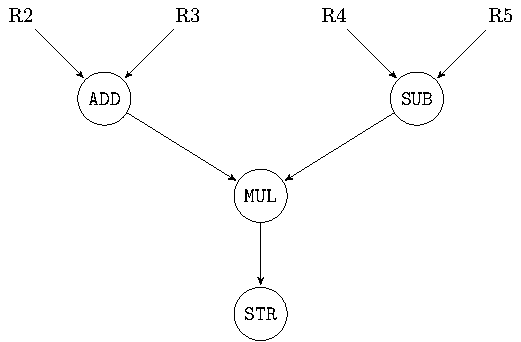
\includegraphics{diagrams/data-flow.pdf}
  \caption{A sample data flow graph.}
  \label{data-flow}
\end{figure}

Though this is a simple example, analysis has shown that it is not uncommon for
real programs to have up to four instructions that can be parallelised at some
point in the program's running time. Obviously, the amount of times when two or
three instructions could be parallelised will be greater than that of four.

In order to exploit this parallelism, we can:

\begin{itemize}
  \item Fetch multiple (in our case two for simplicity) instructions per cycle.
  \item Have multiple ALU's to execute instructions in parallel.
  \item Have common registers and caches, since the instructions are operating
  on the same data.
\end{itemize}

Now we could have an architecture looking like that in Figure~\ref{superscalar}.

\begin{figure}[ht]
  \centering
  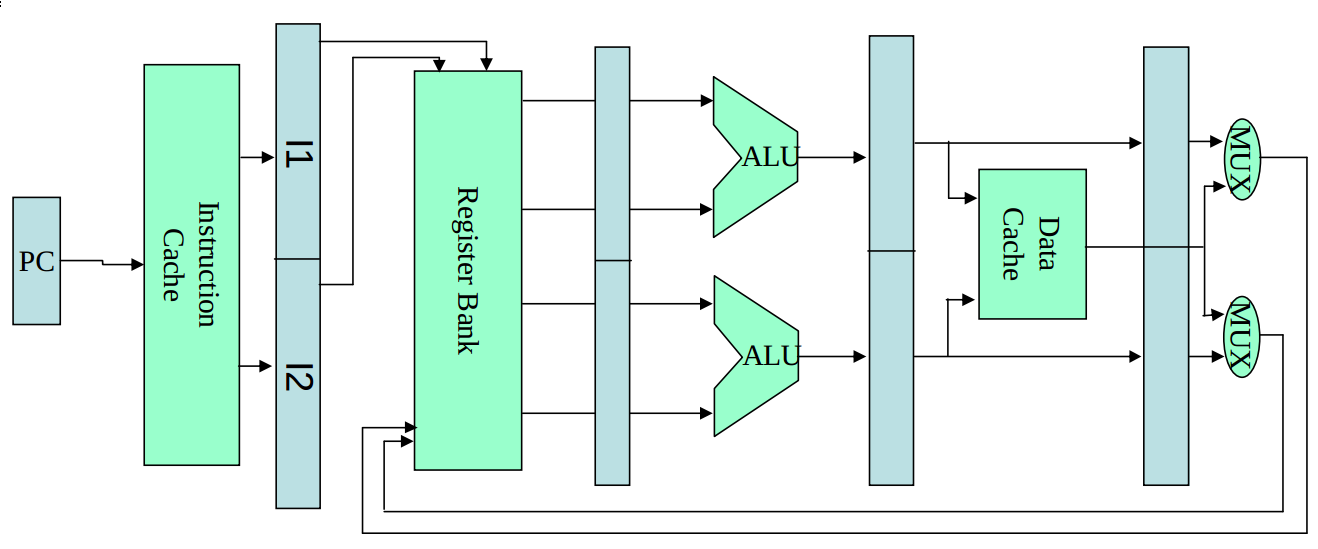
\includegraphics[width=\textwidth]{images/superscalar}
  \caption{A simple superscalar (implementing ILP) architecture.}
  \label{superscalar}
\end{figure}

\marginpar{Note, these multiple reads and writes will be occurring in different
parts of the register bank and cache, since the parallel instructions are (by
nature) independent of each other.}

If we are able to run multiple instructions at the same time, then our registers
and caches are going to have (in this case, which is a low level of parallelism)
roughly twice the load that they had previously. In order to allow them to handle
this extra load, we can make them \textbf{dual ported}, which means that the
access circuitry is duplicated so multiple reads and writes can happen
simultaneously.

In order to implement ILP, we also need a `dispatch unit' in hardware which is
part of the fetch stage (\texttt{IF}). This will fetch multiple instructions if
they are independent and be executed in parallel.

\subsubsection{Out of Order Execution}

In order to get the maximum number of ILP compatible instruction sequences in a
program, the compiler may be able to re-order instructions so that they have a
reduced number of interdependencies. One technique that is based on this is the
Very Long Instruction Word, where each word will be longer than a normal word
(maybe 48, 64 or more bits), and will contain more than one instruction.

Having the compiler re-order instructions means that it will sometimes add
\texttt{NOP}'s into the code, which can increase the binary size, and bloat the
code. The alternative it to rely on expensive hardware to detect out of order
opportunities at runtime.

To implement an out of order processor, you need to have a buffer that
instructions are fetched into, a scheduler to choose which (non-conflicting)
instructions to execute at what times, and a cache to store memory and register
accesses until all the instructions have finished so that the application can
execute normally as though all instructions executed in serial. Figure~\ref{out-
of-order} shows how this could all be implemented.

\begin{figure}[H]
  \centering
  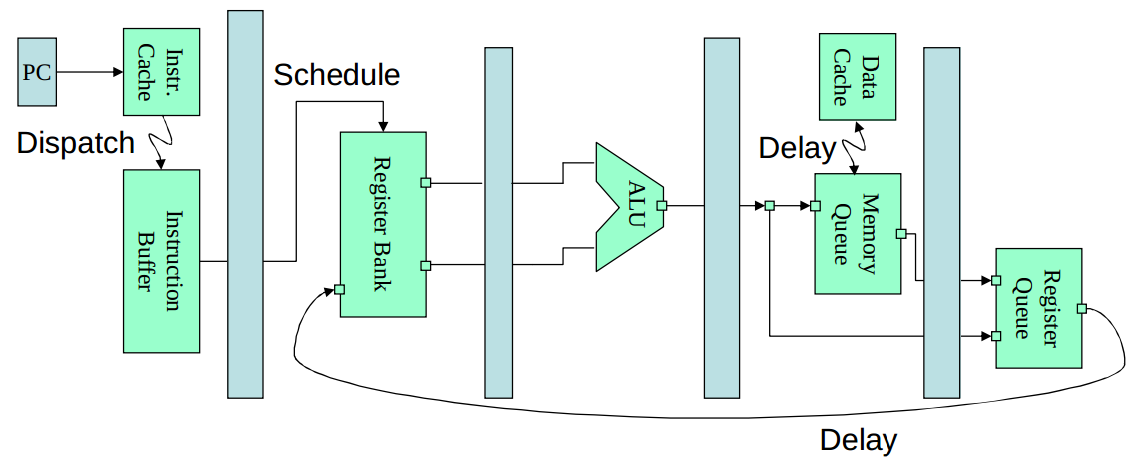
\includegraphics[width=\textwidth]{images/out-of-order}
  \caption{An example of how an out-of-order processor could be implemented.}
  \label{out-of-order}
\end{figure}

\subsubsection{Programmer assisted ILP}

Some processors now support SIMD (Single Instruction Multiple Data)
instructions, that allow one instruction to be executed on multiple
registers/memory locations etc. This is very useful when doing mathematical
computation with stuff like vectors and matrices, since it requires a lot of
repetitive operations that lend themselves easily to parallelism.

One example of this is the \texttt{UADD8} ARM instruction. It adds two registers
together into a third register like a normal add, but it does this four times;
once for each eight bit chunk in the registers. For example, \texttt{UADD8 R0,
R1, R2} will do:

\begin{figure}[H]
  \centering
  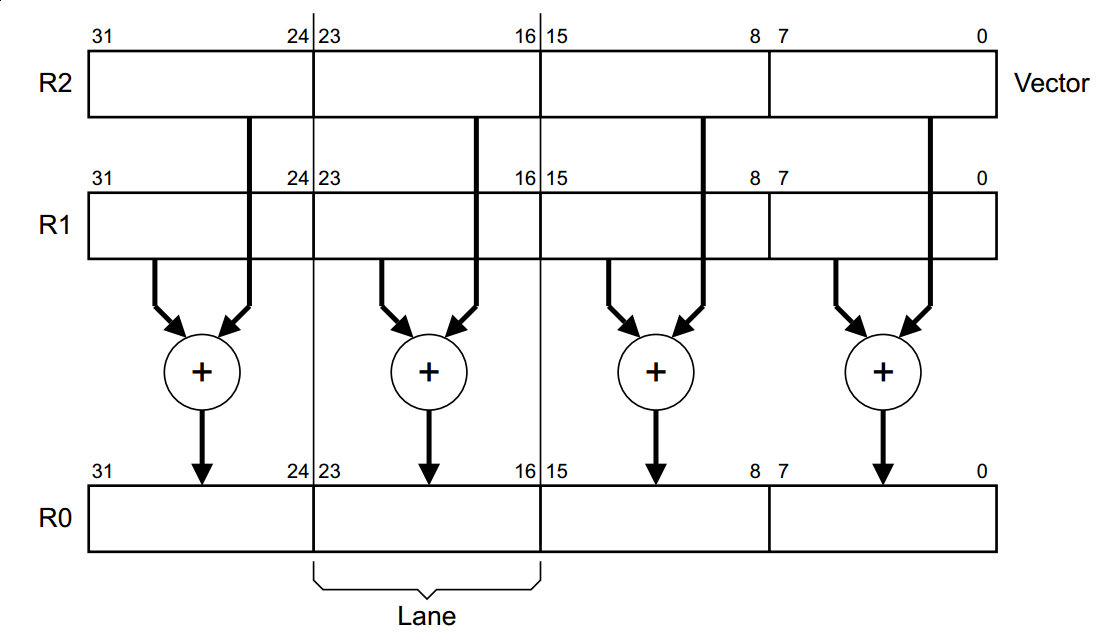
\includegraphics[width=\textwidth]{images/UADD8}
  \caption{A 4 way 8-bit integer add operation.}
  \label{UADD8}
\end{figure}

\section{Multi-Threading}

We have already seen, there are many different ways of increasing CPU
performance:

\begin{itemize}
  \item Increasing the clock frequency
  \item Increasing the \textit{ips} (instructions per clock)
  \item Minimising the impact of accessing memory with a cache
  \item Minimising bubbles (branch prediction)
  \item Minimising bubbles (out of order execution)
  \item Parallelising instructions (with an superscalar architecture)
  \item[ ] \hspace{-2.2em}And, up to a point
  \item Lengthening the pipeline
\end{itemize}

We have said that increasing the parallelism will speed up our pipeline, but in
order to do this, we need to find enough instructions to safely parallelise at
once. There are multiple ways to do this too:

\begin{itemize}
  \item When we get a branch instruction, do we pause until we evaluate the
  outcome of the branch, or keep issueing instructions? If we're using branch
  prediction, then we can keep issueing instructions.

  \item After a cache miss, we need to wait for a certain amount of time for the
  data we want to come from the memory, over the bus and into the CPU. While
  we're waiting, can we carry on issuing other instructions?

  \item Process instructions in parallel (e.g. with a superscalar architecture).

  \item Write to registers while the previous write is pending?
\end{itemize}

These ways of increasing parellism are good, but assume we have only one source
of instructions. However in reality, a CPU will be executing code from multiple
processes at once. What about if we run out of instructions to execute in one
program, we could just context switch to another!

\subsection{Context switch}

In a context switch, the Operating System must load/store a lot of data about
the switching processes:

\begin{mymulticols}
  \begin{itemize}
    \item Process ID
    \item Process state
    \item Program Counter
    \item Stack Pointer
    \item General registers
    \item Memory management information
    \item Open file list (and positions)
    \item Network connections
    \item CPU time used
    \item Parent process ID
  \end{itemize}
\end{mymulticols}

\subsection{Hardware multithreading}

We could have two PC's, two sets of registers (GPR's on the diagram), two
virtual address mappings etc, and have the CPU support multi threading natively.
This would require the OS to be able to handle multiple processors, since the
easiest way of making it work is to make the one processor core look like two
processor cores (since the inputs and outputs are effectively doubled).

\begin{figure}[H]
  \centering
  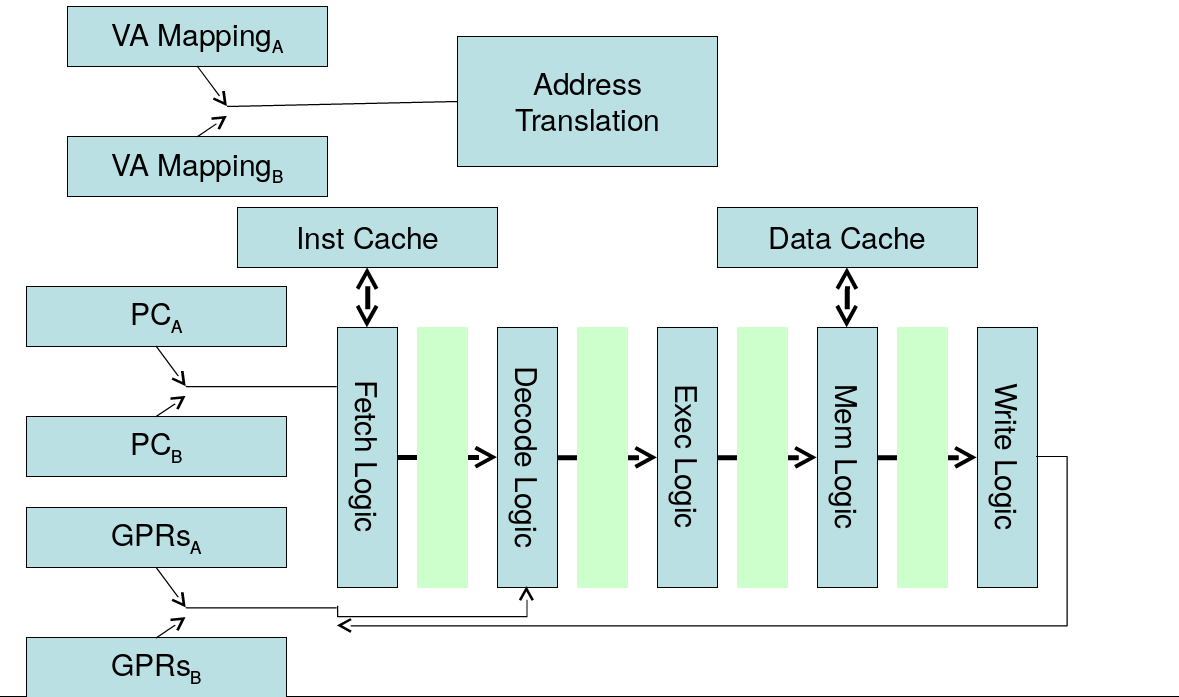
\includegraphics[width=\textwidth]{images/hyperthreading}
  \caption{The architecutre of a multithreaded CPU}
  \label{hyperthreading}
\end{figure}

\section{Multi-Core}

\section{Vitalisation}

\section{Permanent Storage}
